\section{Introduction}
\label{sec:introduction}

% Rise of DL
In recent years, deep learning models have demonstrated superior performance on a variety of tasks \cite{ruede2020multi, brinker2019deep, nguyen2020super}. While performance is still increasing and more tasks are being handled, their performance comes at the cost of complexity: models often use millions to billions of parameters to achieve universal function approximation.
This complexity means that they remain black boxes that cannot be interpreted even by experts.

\blfootnote{Code for replications and experiments will be made available on \url{https://github.com/verenaHeusser/adversarial_interpretation_manipulation}}
\blfootnote{All figures in this article are produced by the author unless noted otherwise.}

% rise of XAI
Such a black box is able to predict fairy well for unseen yet similar data, answering the question of \textit{what} is the most likely label for an input sample. However, most models will provide no answer to \textit{why} or \textit{how} the model chose this label for the instance and which features of the instance were crucial for making this prediction. For example, if a machine learning model is tasked with classifying images of cats (as in \autoref{fig:bb}), one would like to assume that the presence (or absence) of a cat in an image is indicative (contraindicative) of the classification of the image into the "cat" ("not cat") category.

\begin{figure}[t]
    \centering
    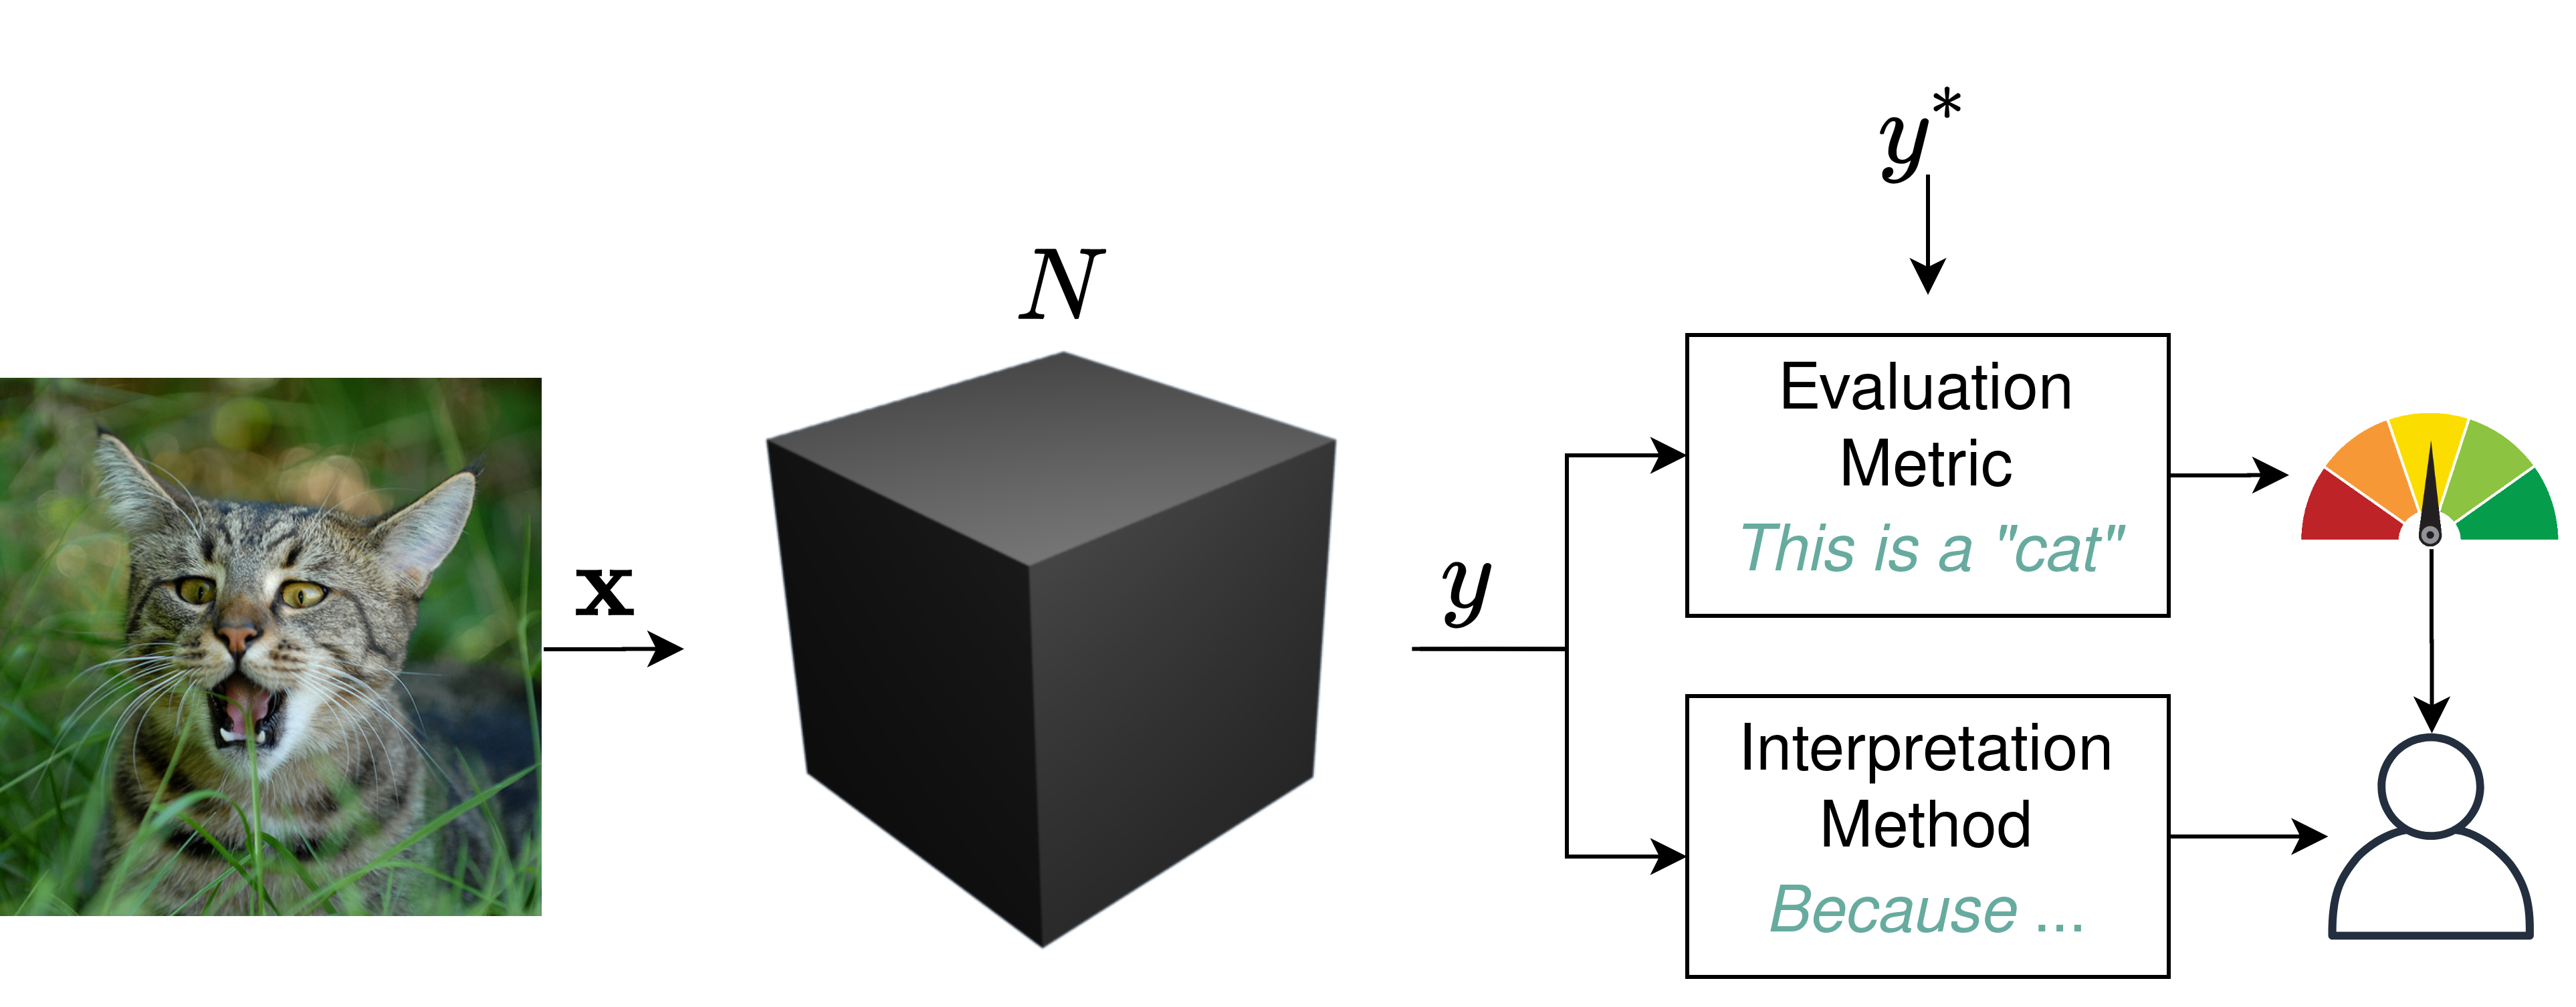
\includegraphics[width=\linewidth]{figures/bb_cat.png}
    \caption{Prediction pipeline using a machine learning model, depicted as a black box. Typically, evaluation metrics require the prediction $y$ and the ground truth label $y^*$ allowing for the assessmant of the model's accuracy. Additionally answering the question \textit{why}, i.e. making the model interpretable for a human, requires additional methods.}
    \label{fig:bb}
    \vspace{-0.3cm}
\end{figure}

Automated algorithms are already in use in critical areas, such as medicine, chemistry, the criminal justice system, the financial sector or the piloting of self-driving cars \cite{chouldechova2017fair, elshawi2019interpretability, whitmore2016mapping}. % med, med, chemistry
Thus, as machine learning models are moving out of the lab into the real-world, the inability of humans to understand these (black box) models seems even more problematic. Not knowing how a model makes predictions, and not being able to detect systematic biases in the model, prevents the vastly advancing technology of machine learning from being used in highly sensitive and safety-critical applications.  

Suppose a deep neural network predicts the risk for cancer from a mammogram, which is an image of breast tissue. A doctor would only use the algorithm if there is a way to validate that (1) the algorithm is accurate (which can be measured in terms of the predictive accuracy), and (2) if the model is also using the correct indications in the data for predicting the risk of cancer. (1) is the standard approach for validating the performance of machine learning models, but in this example, one can clearly see why predictive accuracy might not be enough in many areas. For approaching (2), i.e. uncovering \textit{why} a model predicts a low / high risk of cancer, the research field of explainable artificial intelligence (XAI) offers a fast growing number of methods. Some research even suggests to allow 'peeking inside the black box' of deep learning models \cite{adadi2018peeking}.  

%%%%%%%%%%%%%%%%%%
% In addition to this insecurity on the model level, it is likely that machine learning systems in deployment will be attacked. 

%%%%% iai
The threats of adversarial attacks on deployments of machine learning models has contributed to the field of XAI comprising topics of (1) \textit{model interpretations}, (2) \textit{adversarial attacks}, or manipulation methods and (3) the field of \textit{adversarial manipulations of model interpretations}. All these subfields have the common goal to make models more robust and safe for deployment. 
(1) refers to the development of techniques that can be used to understand and explain the decision making process of a machine learning model or even the development of models that are inherently interpretable. (2) is the field of detecting vulnerabilities in models that cause these models to be deceived by altered input. 
(3) is the main topic of this paper, i.e. how to fool interpretation methods in order to detect vulnerabilities and malfunctions in interpretation methods. 
%%%% 
Ideally, an interpretation or explanation method should indicate which features in the input to a model contribute to the prediction and also to what extent each feature contributes. This notion of extent is often called the \textit{importance} score of a feature. \autoref{fig:lrp_cat} shows such a feature importance map (\autoref{fig:lrp_cat_lrp}) produced by the interpretation method LRP \cite{bach2015pixel} applied to the neural network model Inception-v3 \cite{szegedy2016rethinking}. The input image is from the ImageNet dataset \cite{ILSVRC15}. The output of the interpretation method is projected onto the original image for better human readability. This importance map suggests that specific portions of the original cat image are important for the neural network make the high-confidence prediction (see..) of the category 'tiger cat'. 

\begin{figure}[ht]
    \centering
    \begin{subfigure}{0.32\linewidth}
      
\includegraphics[width=\linewidth]{figures/cat.JPEG}
      \caption{Original.}
      \label{fig:lrp_cat_orig}
    \end{subfigure}
    \begin{subfigure}{0.32\linewidth}
      
\includegraphics[width=\linewidth]{figures/lrp_cat_heatmap.png}
      \caption{Map.}
      \label{fig:lrp_cat_lrp}
    \end{subfigure}
    \begin{subfigure}{0.32\linewidth}
      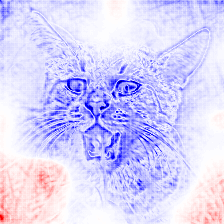
\includegraphics[width=\linewidth]{figures/foolignns/location fooling lrp/lrp_epoch6_no-7.png}
      \caption{Fooled Map.}
      \label{fig:lrp_cat_fooled_lrp}
    \end{subfigure}
    % \begin{subfigure}{0.8\linewidth}
    %     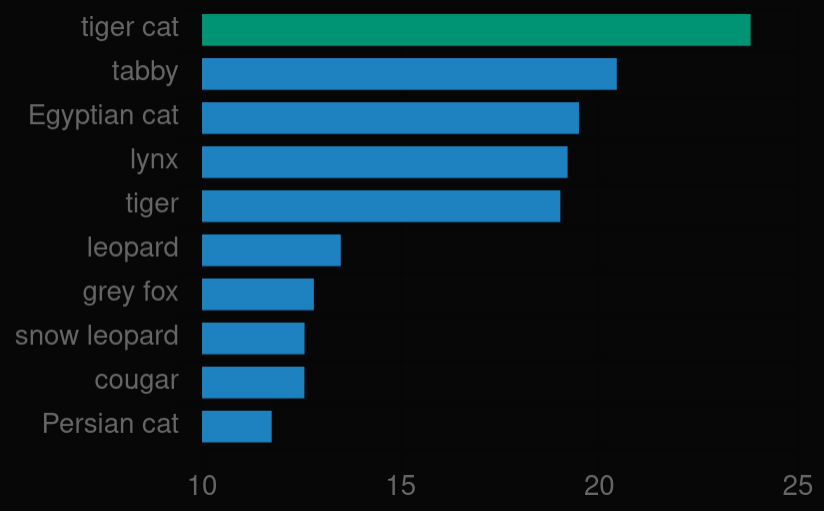
\includegraphics[width=\linewidth]{figures/cat_classification.png}
    %     \caption{Predictive accuracy.}
    %     \label{fig:cat_classification}
    % \end{subfigure}
    \caption{Visualization of the feature importance and fooled feature importance maps produced py the LRP interpreter applied to the image of a cat and an image classification model. The fooling method is the \textit{location} fooling from \cite{fooling_nn_interpreters}. Dark red here means a stronger significance of the feature.}\label{fig:lrp_cat}
    \vspace{-0.3cm}
\end{figure}

% https://towardsdatascience.com/interpretability-in-machine-learning-70c30694a05f 
% biases in ml models - boils down to data

% https://dl.acm.org/doi/pdf/10.1145/3387514.3405859?casa_token=lCc16GOTZsEAAAAA:gypLNU1o2Wwl3wt_b8stRbb0mgxEomX8PWprPeciNdkhVften3-5E01RM50e0W9NGQaGd4TrLOhA

While interpretation methods are already used for analysis of computer vision systems \cite{bach2015pixel, simonyan2013deep, zeiler2014visualizing}, text and sequence analysis \cite{ancona2017towards, arras2017relevant}, and deep learning in security \cite{evaluating_explanations_security}, there is still a lack in the the understanding of model interpretation methods. 
Recent work has shown, that humans are not able to benefit much from interpretation techniques: They cannot build better models and improve their own performance \cite{hase2020evaluating}, are not better at detecting false model decisions even in transparent models \cite{poursabzi2018manipulating}, and even data scientists over-trust and misuse model interpretation methods \cite{kaur2020interpreting}. 
Methodologically, it is unclear how the variety of proposed model interpretation methods are related and what common concepts can be used to evaluate and compare them. Many works are dedicated to establish a formal definition of what it means for a model to be interpretable, and how to select and evaluate methods for generating interpretations of machine learning models \cite{murdoch2019definitions, lipton2018mythos}. However, a growing number of researchers also focus on breaking these interpretation methods, similar to research on adversarial attacks on machine learning models, which is deeply fueled by the vast deployment of models in the real world \cite{fooling_nn_interpreters,ghorbani2019interpretation,dimanov2020you,dombrowski2019explanations,advlime_aies20, le2020remote, zhang2020interpretable, kuppa2020black, anders2020fairwashing, lakkaraju2020fool, kindermans2017reliability}.

% %%%%%%%%%%%%%%%%%%%%%%%%%%%%%%%%%%%%%%%%%%%%%%
% \subsection{Why is Interpretability Important?}
% \label{subsec:importance_of_interpretability}

% First, interpretability is helpful as it can help to build trust in a machine learning application. 
% % Suppose a neural network predicts the risk for cancer from a mammogram, which is an image of breast tissue. A doctor would only use the algorithm if there is a way to validate that (1) tha algorithm is accurate (which can be measured in terms of the predictive accuracy), and (2) if the model is also using the correct indications in the data for predicting the risk of cancer. (1) is the standard approach for validating the performance of machine learning models, but in this example, one can clearly see why predictive accuracy might not be enough. For approaching (2), i.e. uncovering \textit{why} a model predicts a low / high risk of cancer, a variety of interpretation methods are proposed.  
% % Ideally, an interpretation, or explanation method should indicate which pixels in the original image contribute to the prediction and also to what extent each pixel contributes. The extent to which each pixel contributes to a prediction is often called the \textit{importance} score of a feature. 

% The advantage of post-hoc interpretations is that they do not interfere with the training process of the model, and thus do not change the model. As the name says, post-hoc means that the techniques can be easily applied to an already trained model without much further computational overhead. 

% % https://thegradient.pub/interpretability-in-ml-a-broad-overview/ intro motvation
% % https://towardsdatascience.com/why-how-interpretable-ml-7288c5aa55e4 also

% High interpretability is desired as it can help to to uncover biases in the model. Suppose a machine learning model is to be deployed for the task of income prediction based on features such as age, race, gender, education and hours of work per week. The performance of the system would mainly be evaluated in terms oft the predictive accuracy and the fairness of the system. The former can be evaluated with metrics, such as accuracy on a held-out test set. For the latter, interpretability methods might be applied to observe which input features are used by the model to predict the income. 
% % TODO note here that tha data from adult_income do actually not allow for these features to be more important than others. 
% If the model uses sensitive features, such as sex and race as important features, it is systematically biased and thus unfair. 

%%%%%%%%%%%%%%%%%%%%%%%% Outline
\mypar{Outline. }\newline
This article examines a topic at the intersection of interpretable and adversarial machine learning research. 
The overview presented in this article examines the existing literature and contributions in the field of XAI focusing on methods to manipulate explanation methods. We try to offer a comprehensive taxonomy of these interpretation manipulation methods. 

This paper is structured as follows. \autoref{sec:interpretation_methods} introduces common interpretation methods for machine learning models, and offers a taxonomy of the variety of techniques and a brief outline of popular interpretation methods.
In \autoref{sec:manipulation_methods}, the main topic of this paper, namely manipulation methods for deceiving interpretation techniques, is outlined. A taxonomy of methods is proposed and possible evaluation criteria are listed. \autoref{sec:benchmarking} proposes approaches to benchmark the robustness of interpretation techniques and \autoref{sec:manipulations} provides a review of important studies in the field of manipulation methods. The implications of this research area on XAI are discussed in section \autoref{sec:discussion}.